\begin{minipage}{0.75\linewidth}
\begin{figure}[h]
    \centering
    \begin{adjustbox}{max width=1.0\linewidth, keepaspectratio}
        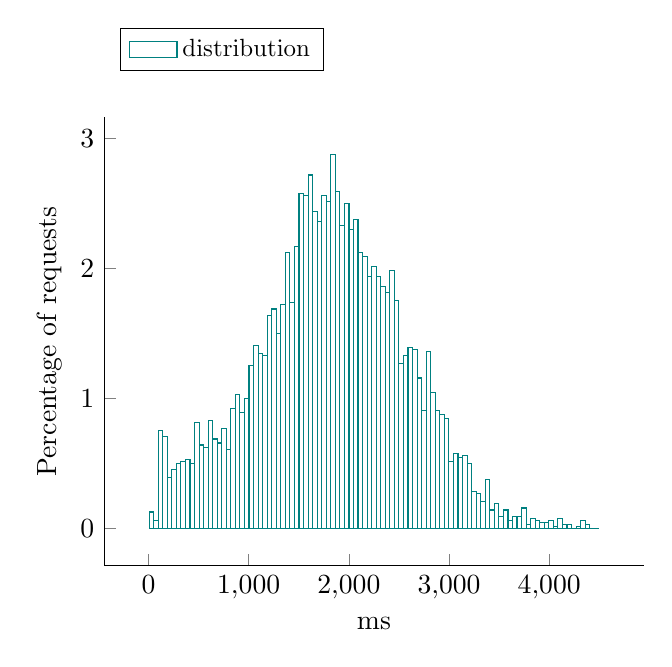
\begin{tikzpicture}
            \begin{axis}[ylabel = Percentage of requests, 
xlabel = ms, 
legend style = {nodes={scale=0.9, transform shape}, at={(0.03,1.2)}, anchor=north west, draw=black, fill=white, align=left, legend columns=3},
area style, mark size = 0pt,
 cycle list name = exotic,
  axis lines* = left]
		\addplot +[ybar interval] coordinates {
			 (6, 0.125)
			 (51.34, 0.0625)
			 (96.68, 0.75)
			 (142.02, 0.703125)
			 (187.36, 0.390625)
			 (232.7, 0.453125)
			 (278.04, 0.5)
			 (323.38, 0.515625)
			 (368.72, 0.53125)
			 (414.06, 0.5)
			 (459.4, 0.8125)
			 (504.74, 0.640625)
			 (550.08, 0.625)
			 (595.42, 0.828125)
			 (640.76, 0.6875)
			 (686.1, 0.65625)
			 (731.44, 0.765625)
			 (776.78, 0.609375)
			 (822.12, 0.921875)
			 (867.46, 1.03125)
			 (912.8, 0.890625)
			 (958.14, 1)
			 (1003.48, 1.25)
			 (1048.82, 1.40625)
			 (1094.16, 1.34375)
			 (1139.5, 1.32812)
			 (1184.84, 1.64062)
			 (1230.18, 1.6875)
			 (1275.52, 1.5)
			 (1320.86, 1.71875)
			 (1366.2, 2.125)
			 (1411.54, 1.73438)
			 (1456.88, 2.17188)
			 (1502.22, 2.57812)
			 (1547.56, 2.5625)
			 (1592.9, 2.71875)
			 (1638.24, 2.4375)
			 (1683.58, 2.35938)
			 (1728.92, 2.5625)
			 (1774.26, 2.51562)
			 (1819.6, 2.875)
			 (1864.94, 2.59375)
			 (1910.28, 2.32812)
			 (1955.62, 2.5)
			 (2000.96, 2.29688)
			 (2046.3, 2.375)
			 (2091.64, 2.125)
			 (2136.98, 2.09375)
			 (2182.32, 1.9375)
			 (2227.66, 2.01562)
			 (2273, 1.9375)
			 (2318.34, 1.85938)
			 (2363.68, 1.8125)
			 (2409.02, 1.98438)
			 (2454.36, 1.75)
			 (2499.7, 1.26562)
			 (2545.04, 1.32812)
			 (2590.38, 1.39062)
			 (2635.72, 1.375)
			 (2681.06, 1.15625)
			 (2726.4, 0.90625)
			 (2771.74, 1.35938)
			 (2817.08, 1.04688)
			 (2862.42, 0.90625)
			 (2907.76, 0.875)
			 (2953.1, 0.84375)
			 (2998.44, 0.515625)
			 (3043.78, 0.578125)
			 (3089.12, 0.546875)
			 (3134.46, 0.5625)
			 (3179.8, 0.5)
			 (3225.14, 0.28125)
			 (3270.48, 0.265625)
			 (3315.82, 0.203125)
			 (3361.16, 0.375)
			 (3406.5, 0.140625)
			 (3451.84, 0.1875)
			 (3497.18, 0.09375)
			 (3542.52, 0.140625)
			 (3587.86, 0.0625)
			 (3633.2, 0.09375)
			 (3678.54, 0.09375)
			 (3723.88, 0.15625)
			 (3769.22, 0.03125)
			 (3814.56, 0.078125)
			 (3859.9, 0.0625)
			 (3905.24, 0.046875)
			 (3950.58, 0.046875)
			 (3995.92, 0.0625)
			 (4041.26, 0.015625)
			 (4086.6, 0.078125)
			 (4131.94, 0.03125)
			 (4177.28, 0.03125)
			 (4222.62, 0)
			 (4267.96, 0.015625)
			 (4313.3, 0.0625)
			 (4358.64, 0.03125)
			 (4403.98, 0)
			 (4449.32, 0)
			 (4494.66, 0.015625)
		};
\addlegendentry{distribution};
           \end{axis}
      \end{tikzpicture}
  \end{adjustbox}
  \caption{Response time distribution - req = ReadTimeline-1}
\end{figure}
\end{minipage}\hfill\begin{minipage}{0.18\linewidth}
\begin{table}[h]
\begin{tabular}{|cc|}
\hline
\textbf{} & \textbf{ms}\\ \hline
 \Xhline{0.005\arrayrulewidth}
min & 6\\
 \Xhline{0.005\arrayrulewidth}
max & 4540\\
 \Xhline{0.005\arrayrulewidth}
mean & 1819\\
 \Xhline{0.005\arrayrulewidth}
std & 752\\
\hline
\hline
 \Xhline{0.005\arrayrulewidth}
25th & 1344\\
 \Xhline{0.005\arrayrulewidth}
50th & 1826\\
 \Xhline{0.005\arrayrulewidth}
75th & 2323\\
 \Xhline{0.005\arrayrulewidth}
80th & 2446\\
 \Xhline{0.005\arrayrulewidth}
85th & 2601\\
 \Xhline{0.005\arrayrulewidth}
90th & 2789\\
 \Xhline{0.005\arrayrulewidth}
95th & 3030\\
 \Xhline{0.005\arrayrulewidth}
99th & 3595\\
\hline
\end{tabular}
\caption{Response time}
\end{table}
\end{minipage}\hfill